\documentclass[12pt]{article}
\usepackage[a4paper, total={7.5in, 11in}]{geometry}

%\usepackage{array}
\usepackage{graphicx, subfig, wrapfig }
\newcommand\headerMe[2]{\noindent{}#1\hfill#2}









\begin{document}

\headerMe{Royaume du Maroc}{année scolaire \emph{2021-2022}}\\
\headerMe{Ministère de l'Éducation nationale, }{  Professeur :\emph{Zakaria Haouzan}}\\
\headerMe{du Préscolaire et des Sports}{Établissement : \emph{Lycée SKHOR qualifiant}}\\

\begin{center}
Devoir N°2 \\
    Filière Tronc Commun Scientifique\\
Durée 2h00
\\
    \vspace{.2cm}
\hrulefill
\Large{Chimie }
\hrulefill\\
    \emph{Les deux parties sont indépendantes}
\end{center}
%end Headerss------------------------

%      \end{wrapfigure}





%__________________Chimie ______________________-
%%%%%%%+_+_+_+_+_+_+_+_+_Partie1

 \section*{Partie 1 : synthèse de l’éthanoate de linalyle}
            \begin{wrapfigure}[12]{r}{0.25\textwidth}
            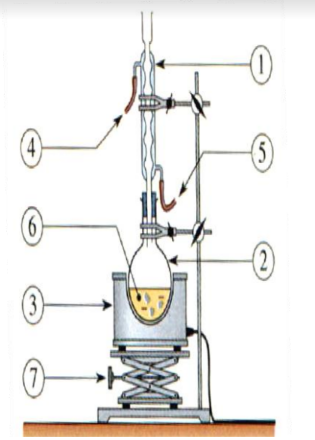
\includegraphics[width=0.25\textwidth]{./img/img00.png}
            \end{wrapfigure}
1.  Définir la synthèse d’une espèce chimique
\\2. Donner le nom de la technique
\\3. Légender le schéma du montage expérimental
\\4. Quelle est l’utilité de la technique
\\5. Quel est le rôle du réfrigérant et de la pierre ponce
\\6. Quels sont les réactifs utilisés pour la synthèse de l’éthanoate de linalyle,
préciser les conditions de la synthèse.
\\7. Pourquoi le réfrigérant à boules doit-il rester ouvert à son extrémité
supérieure ?
\\8. Nommer les trois étapes de la synthèse.
\\9. Donner deux méthodes permettant de vérifier la pureté de l’espèce
chimique synthétisée

\section*{Partie 2 : Le modèle de l'atome}
Remplir le tableau suivant :

    \begin{center}
    \begin{tabular} { | c | c | c |c|c| }
    \hline\hline
        Symbole         & $^{16}_8O$ &$^{12}_6C$ & $^{23}_{11}Na^{+}$ & $^{32}_{...}S^{...}$\\\hline
        Nombre de protons & & & & \\\hline
        Nombre de neutons & & & & \\\hline
        Nombre de nuléons & & & & \\\hline
        Nombre d’électrons& & & & 18\\\hline
        Structure électronique & & & & \\\hline
        Charge Totale & & & &-2e \\\hline
    \hline
    \end{tabular}
    \end{center}
    1. Le symbole de l’élément chimique bismuth est Bi. Le noyau de son atome est
constitué de 209 nucléons et sa charge est $Q = 1,33.10^{-17}C$
\\1.a) Déterminer le numéro atomique Z de l’atome du bismuth.
\\1.b) Donner le symbole de cet atome.
\\1.c) Calculer sa masse approchée.
\\2. Le symbole de l’élément chimique phosphore est P. Le noyau de
son atome est constitué de 15 protons et de 16 neutrons.
\\2.a) Donner le symbole de cette atome.
\\2.b) La structure électronique de l’ion phosphure est : $(K)^2(L)^8(M)^8$ Donner le symbole de cet ion

Donneés : $e = 1.6.10^{-19} C$;  $mp=mn=1.67.10^{-27}Kg$
%_____________________________________PHYSIque Partie 22222____________________________________________________________________________
\begin{center}
    \vspace{3cm}
\hrulefill
\Large{Physique }
\hrulefill\\
    \emph{Les deux parties sont indépendantes}
\end{center}
%end Headerss------------------------

 \section*{Partie 1 :Le mouvement }
   %  \begin{wrapfigure}[12]{r}{0.25\textwidth}
    %        \end{wrapfigure}
On enregistre les positions occupées par un point M d’un solide en
mouvement sur une table à coussin d’air pendant des intervalles de
temps égaux à $\tau = 40 ms$ , on obtient l’enregistrement suivant :
\begin{center}
            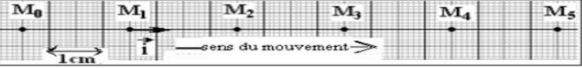
\includegraphics[width=0.75\textwidth]{./img/img01.png}
\end{center}
\begin{enumerate}
\item Quelle est la nature du mouvement du point M ? justifier.
\item Calculer la valeur de la vitesse moyenne de M entre les points $M_1$ et $M_4$.
\item Calculer la valeur de la vitesse instantanée aux points $M_1$ et $M_2$
\item Représenter $V_2$ en choisissant l’échelle : $0,25m/s \rightarrow 1cm$.
\item En considérant le point M1 comme origine des abscisses et l’instant de
l’enregistrement du point M3 comme origine des dates.
        \begin{enumerate}
               \item Complétez le remplissage du tableau suivant :
 \begin{center}
    \begin{tabular} { | c | c | c |c|c| }
    \hline\hline
        Position & $M_0$ & $M_1$ & $M_2$ & $M_3$\\\hline
        x(cm)    & & & & \\\hline
        t(s)     && & & \\\hline
    \hline
    \end{tabular}
    \end{center}
\item Ecrire l’équation horaire du mouvement de M .
        \end{enumerate}
\end{enumerate}

 \section*{Partie 2 :Principe d’inertie :  }
         \begin{wrapfigure}{r}{0.4\textwidth}
        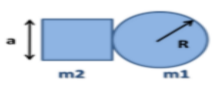
\includegraphics[width=0.2\textwidth]{./img/img02.png}
    \end{wrapfigure}

          1 . Enoncé le principe d’inertie.
          \\2 . On considère le système formé de deux corps homogènes.
                \\Un disque de rayon R= 20 cm et de masse $m_1$.
                \\Un carré de côté a= 10 cm et de masse $m_2$ =$m_1$/4
                \\Déterminer la position du centre d'inertie G du système

\end{document}
